\let\negmedspace\undefined
\let\negthickspace\undefined
\documentclass[journal,12pt,onecolumn]{IEEEtran}
\usepackage{cite}
\usepackage{amsmath,amssymb,amsfonts,amsthm}
\usepackage{algorithmic}
\usepackage{graphicx}
\usepackage{textcomp}
\usepackage{xcolor}
\usepackage{txfonts}
\usepackage{listings}
\usepackage{enumitem}
\usepackage{mathtools}
\usepackage{gensymb}
\usepackage{comment}
\usepackage[breaklinks=true]{hyperref}
\usepackage{tkz-euclide} 
\usepackage{listings}
\usepackage{gvv}                                        
\def\inputGnumericTable{}                                 
\usepackage[latin1]{inputenc}                                
\usepackage{color}                                            
\usepackage{array}                                            
\usepackage{longtable}                                       
\usepackage{calc}                                             
\usepackage{multirow}                                         
\usepackage{hhline}                                           
\usepackage{ifthen}                                           
\usepackage{lscape}

\newtheorem{theorem}{Theorem}[section]
\newtheorem{problem}{Problem}
\newtheorem{proposition}{Proposition}[section]
\newtheorem{lemma}{Lemma}[section]
\newtheorem{corollary}[theorem]{Corollary}
\newtheorem{example}{Example}[section]
\newtheorem{definition}[problem]{Definition}
\newcommand{\BEQA}{\begin{eqnarray}}
\newcommand{\EEQA}{\end{eqnarray}}
\newcommand{\define}{\stackrel{\triangle}{=}}
\theoremstyle{remark}
\newtheorem{rem}{Remark}
\begin{document}

\bibliographystyle{IEEEtran}
\vspace{3cm}


\title{Question 41.2023}
\author{EE22BTECH11051}

\maketitle
\vspace{3cm}

\textbf{Question:} \\
Suppose that $X_1$,$X_2$, ...,$X_{10}$ are independen and identically distributed random vectors each having
$N_2(\mu,\Sigma)$ distribution, where $\Sigma$ is non-singular. If
\begin{align}
    \text{U} = \frac{1}{1+(\bar{X} - \mu)^T\Sigma^{-1}(\bar{X} - \mu)} ,
\end{align}
where $\bar X = \frac{1}{10}\Sigma_{i = 1}^{10} X_{i}$ then the value of $\log_e \pr {U \le \frac{1}{2}}$ equals

\begin{enumerate}
    \item -5
    \item -10
    \item -2
    \item -1
\end{enumerate}
\hfill {GATE ST 2023}\\
\textbf{Solution:}\\
We are given a bivariate distribution;
\begin{align}
    X_{i} \sim N_2(\mu,\Sigma)\\
\end{align}
The distribution of $\bar{X}$ can be given as: \\

The mean of $\bar{X}$ will be the average of the means of X1, X2, ..., X10, which is:
\begin{align}
    \mu_{\bar{X}} =\frac{\mu + \mu + \mu + ... + \mu}{10} = \frac{10\mu}{10} = \mu   
\end{align}
And since the distributions $X_1$,$X_2$, ...,$X_{10}$ are independent, the covariance between them is zero. Hence we can find 
the new covariance as:\\
The variance of a sum of i.i.d random variables is calculated as
\begin{align}
    \text{var}\brak{Y_n} &= \text{E}\sbrak{\brak{\frac{1}{n} \sum_{i=1}^{n} X_i}^2} - \brak{\text{E}\sbrak{\frac{1}{n} \sum_{i=1}^{n} X_i}}^2\\
    &= \frac{1}{n^2} \cbrak{\text{E}\sbrak{\brak{\sum_{i=1}^{n} X_i}^2} - \brak{\text{E}\sbrak{\sum_{i=1}^{n} X_i}}^2}
\end{align}
But
\begin{align}
    \text{E}\sbrak{\brak{\sum_{i=1}^{n} X_i}^2} &= \text{E}\sbrak{\sum_{i=1}^{n} \sum_{j=1}^{n} X_iX_j}\\
    &= \sum_{i=1}^{n} \sum_{j=1}^{n} \text{E}\sbrak{X_iX_j} 
\end{align}
and 
\begin{align}
    \brak{\text{E}\sbrak{\sum_{i=1}^{n} X_i}}^2 &= \brak{\sum_{i=1}^{n} \text{E}\sbrak{X_i}}^2\\
    &= \sum_{i=1}^{n} \sum_{j=1}^{n} \text{E}\sbrak{X_i} \text{E}\sbrak{X_j} 
\end{align}
Putting (8) and (10) in (6) , and using the definition of covariance,
\begin{align}
    \text{var}\brak{Y_n} &= \frac{1}{n^2} \cbrak{\sum_{i=1}^{n} \sum_{j=1}^{n} \brak{\text{E}\sbrak{X_iX_j} - \text{E}\sbrak{X_i} \text{E}\sbrak{X_j}}}\\
    &= \frac{1}{n^2} \cbrak{\sum_{i=1}^{n} \sum_{j=1}^{n} \text{cov}\brak{X_i, X_j}} 
\end{align}
As all the variables are i.i.d's and are thus uncorrelated,
\begin{align}
    \text{cov}\brak{X_i, X_j} =
    \begin{cases}
        0 & \text{if } i \ne j\\
        \text{var}\brak{X_i} & \text{if } i = j
    \end{cases}
\end{align}

\begin{align}
    \text{var}\brak{Y_n} &= \frac{1}{n^2} \brak{\sum_{i=1}^{n} \text{cov}\brak{X_i, X_i}}\\
     &= \frac{1}{n^2} \brak{\sum_{i=1}^{n} \text{var}\brak{X_i}}\\
     &= \frac{1}{n^2} \brak{\sum_{i=1}^{n} \Sigma}\\
     &= \frac{\Sigma}{n}
\end{align}
hence;
\begin{align}
    \bar{X} \sim N_2\brak{\mu,\frac{\Sigma}{n}}
\end{align}
Now let us convert this normal distribution into $\chi^{2}_{2}$ distrribution; where $\chi^{2}_{k}$ distribution is given as;
\begin{align}
    f(x) = \frac{x^{\frac{k}{2}-1}}{2^{\frac{k}{2}}\Gamma(\frac{k}{2})} \quad  x \ge 0\\
\end{align}
hence we get;
\begin{align}
    \frac{(\bar{X}-\mu)^T(\bar{X}-\mu)}{\brak{\frac{\Sigma}{n}}} \sim \chi^{2}_{2}
\end{align}
we can now write this as;
\begin{align}
    n(\bar{X} - \mu)^T\Sigma^{-1}(\bar{X} - \mu) \sim \chi^{2}_{2}
\end{align}
Let Y be;
\begin{align}
    Y = n(\bar{X} - \mu)^T\Sigma^{-1}(\bar{X} - \mu)
\end{align}
which follows $\chi^{2}_{2}$ distrribution\\
Now;
\begin{align}
    \pr{U \le \frac{1}{2}}
    &= \pr{\frac{1}{1+\frac{Y}{n}} \le \frac{1}{2}}\\
    &= \pr{\frac{Y}{n} \ge 1}\\
    &= \pr{Y \ge 10}
\end{align}
Since $k=2$ for Y, we get;
\begin{align}
    &= \int_{10}^{\infty} \frac{1}{2}e^{-\frac{y}{2}} \,dy\\
    &= e^{-5}   
\end{align}

Hence;
\begin{align}
    \log_e \pr{U \le \frac{1}{2}} = -5
\end{align}

\textbf{Simulation Steps:}
\begin{enumerate}
    \item Set the number of simulations
    \item Run a loop for number of simulations specified
    \item Generate random vectors from a bivariate normal distribution
    \item Calculate the sample mean and set the covariance matrix
    \item Using the given formula, calculate U for each simulation
    \item Calculate the simulated probability adn take the natural log of that value
\end{enumerate}

\begin{figure}[!ht]
    \centering
    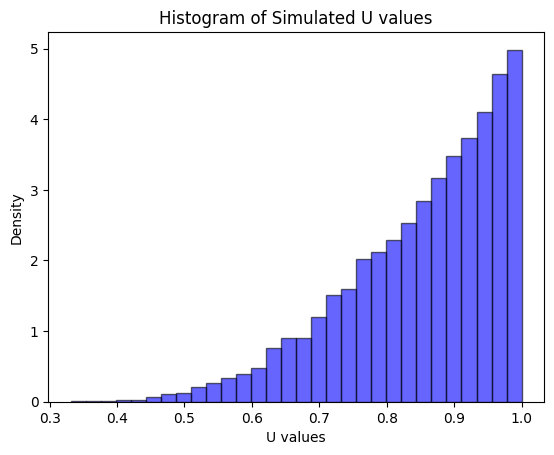
\includegraphics[width=\columnwidth]{./figs/sim.png}
    \caption{Plot of $p_X(n)$.Simulations are close to the analysis. }
    \end{figure}

\end{document}